\documentclass[12pt]{article}

\setlength{\parindent}{0em}
\setlength{\parskip}{.5em}

\usepackage{framed}
\newcounter{problem}
\newcounter{problempart}[problem]
\newcounter{solutionpart}[problem]
\newenvironment{problem}{\stepcounter{problem}\noindent{\bf\arabic{problem}.}}{\setcounter{problempart}{0}\setcounter{solutionpart}{0}}
\newenvironment{solution}{\par\textcolor{blue}\bgroup}{\egroup\par}
\newcommand{\qpart}{\stepcounter{problempart}${}$\\\noindent{(\alph{problempart})} }
\newcommand{\spart}{\stepcounter{solutionpart}${}$\\\noindent{(\alph{solutionpart})} }
\newcommand{\TODO}{\textcolor{red}{$\blacksquare$}}
\newcommand{\SOL}[1]{\textcolor{blue}{#1}}

\usepackage{hyperref}
\usepackage{fullpage}
\usepackage{amsmath,mathabx,MnSymbol}
\usepackage{color,tikz}
\usepackage{footnote,enumitem}
\usepackage{longtable}
\newcommand{\mx}[1]{\begin{pmatrix}#1\end{pmatrix}}
\definecolor{dkgreen}{rgb}{0,.5,0}
\usepackage{algorithm}
\usepackage[noend]{algpseudocode}

\newcommand{\uu}{\mathbf{u}}
\newcommand{\vv}{\mathbf{v}}
\newcommand{\cc}{\mathbf{c}}
\newcommand{\ww}{\mathbf{w}}
\newcommand{\xx}{\mathbf{x}}
\newcommand{\zz}{\mathbf{z}}
\newcommand{\ee}{\mathbf{e}}
\newcommand{\pp}{\mathbf{p}}
\newcommand{\qq}{\mathbf{q}}
\renewcommand{\AA}{\mathbf{A}}
\newcommand{\BB}{\mathbf{B}}
\newcommand{\CC}{\mathbf{C}}
\newcommand{\DD}{\mathbf{D}}
\newcommand{\nn}{\mathbf{n}}
\newcommand{\gp}[1]{\left(#1\right)}

\newcommand{\TODOL}[1]{\textcolor{red}{\underline{\hspace{#1 cm}}}}

\usepackage{listings}

\lstset{
  language=C++,
  showstringspaces=false,
  identifierstyle=\color{magenta},
  basicstyle=\color{magenta},
  keywordstyle=\color{blue},
  identifierstyle=\color{black},
  commentstyle=\color{green},
  stringstyle=\color{red}
}

\begin{document}

\title{CS130 - Lights}
\date{}
\author{Name: \TODOL7\qquad\qquad SID: \TODOL4}
\maketitle
\begin{center}
\end{center}



\begin{problem}
  Modify test case 12.txt so that it produces the following result:\\
  \begin{center}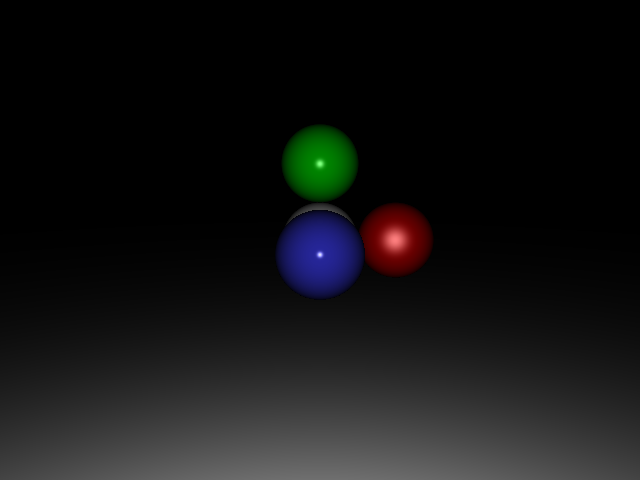
\includegraphics[width=\textwidth]{figures/lights-12-a.png}\end{center}
\end{problem}

\begin{solution}
  \textbf{\textcolor{red}{\TODO}}
\end{solution}

\clearpage
\begin{problem}
  Modify test case 12.txt so that it produces the following result:\\
  \begin{center}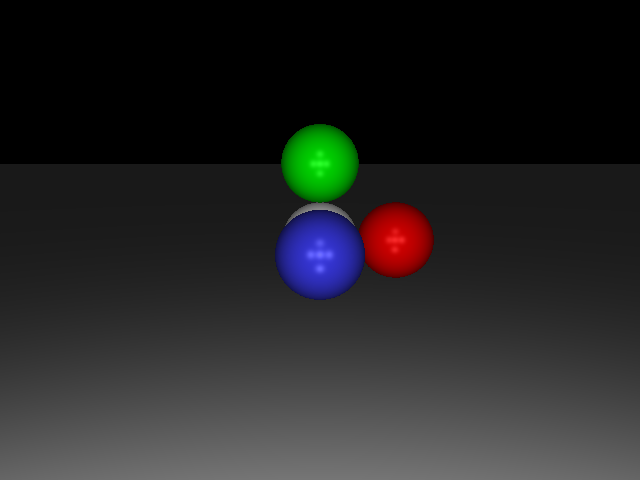
\includegraphics[width=\textwidth]{figures/lights-12-b.png}\end{center}
\end{problem}

\begin{solution}
  \textbf{\textcolor{red}{\TODO}}
\end{solution}

\clearpage
\begin{problem}
  Modify test case 12.txt so that it produces the following result:\\
  \begin{center}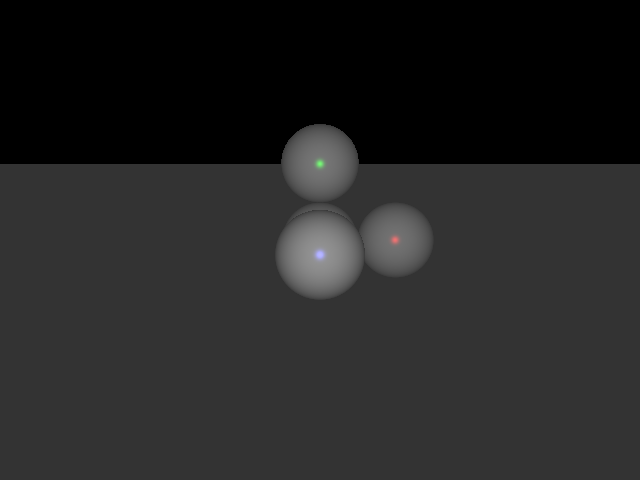
\includegraphics[width=\textwidth]{figures/lights-12-c.png}\end{center}
\end{problem}

\begin{solution}
  \textbf{\textcolor{red}{\TODO}}
\end{solution}

\clearpage
\begin{problem}
  Modify test case 17.txt so that it produces the following result:\\
  \begin{center}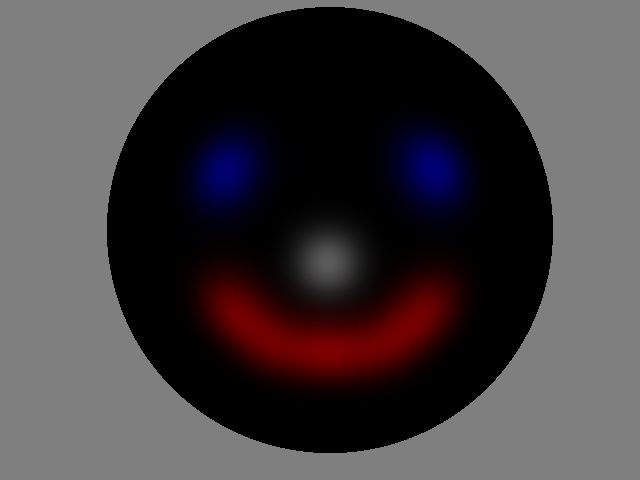
\includegraphics[width=\textwidth]{figures/lights-17-a.png}\end{center}
\end{problem}

\begin{solution}
  \textbf{\textcolor{red}{\TODO}}
\end{solution}

\end{document}

\item types:
  \begin{itemize}
  \item ambient
  \item point
  \item examples of each \hw{hw:rt-lights}
  \end{itemize}
